\label{plugin}
The POP-Java system can be augmented by its users. If the programmer feels the need of a new network protocol or a new encoding protocol, he can create a POP-Java plugin and add it to the system easily. This chapter aims to present the combox and the buffer plugin systems.


\subsection{Combox plugin}
The Combox is the component responsible for the network communication between an application and a parallel object or between two parallel objects. In the current version of POP-Java, only the protocol socket is implemented. If the programmer needs another protocol, he can create his own Combox. \s

To create a new protocol for POP-Java, the programmer needs to create three different classes : a combox, a combox server and a combox factory.\s

The combox must inherits from the super class ComboxPlugin located in the package popjava.combox in the POP-Java library. The figure[\ref{fig:combox_class}] shows the ComboxPlugin class signature. 

\begin{figure}[ht]
\caption{ComboxPlugin class signature}
\center
\label{fig:combox_class}
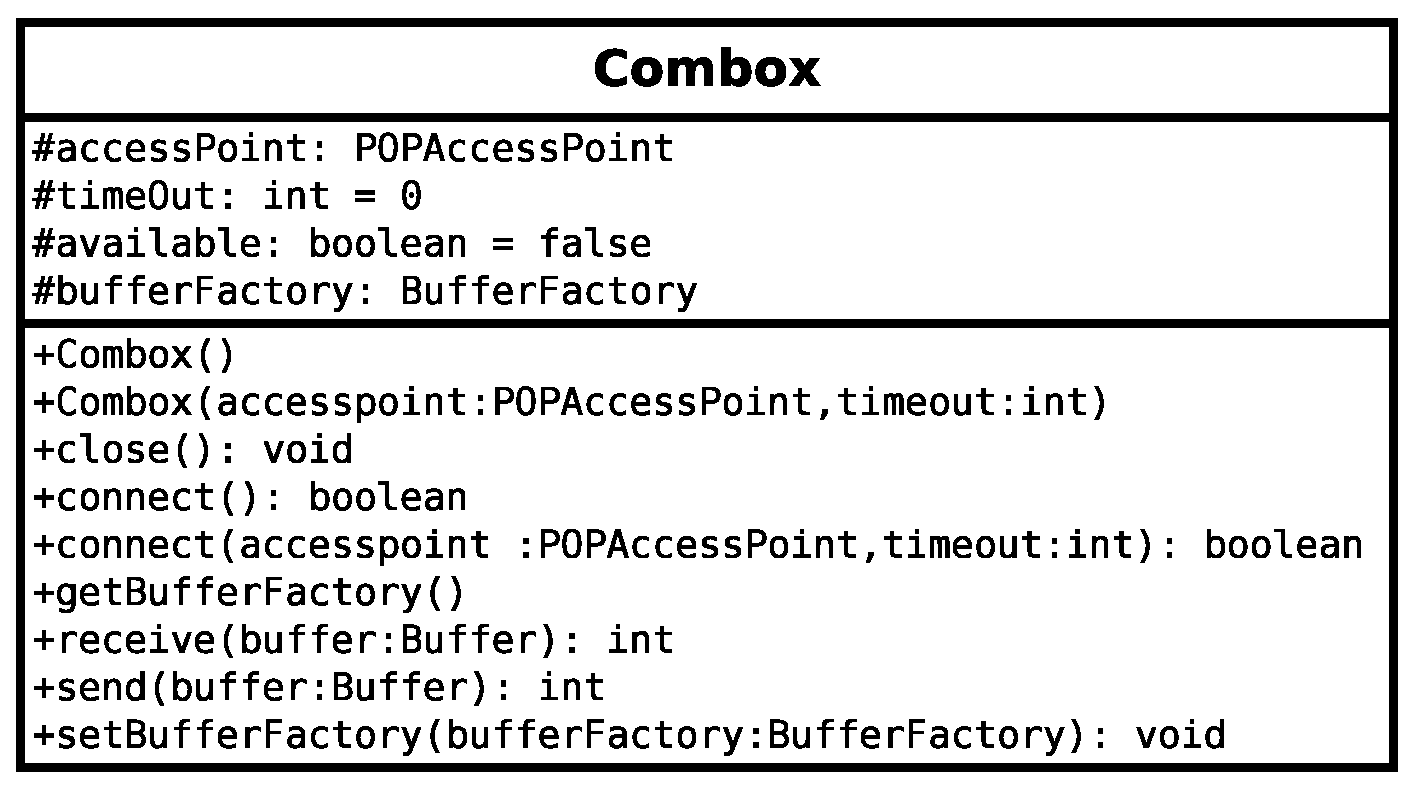
\includegraphics[scale=0.5]{combox.eps}
\end{figure}
\pagebreak

The combox server must inherits from the super class ComboxServer located in the package popjava.combox in the POP-Java library. The figure[\ref{fig:comboxserver_class}] shows the ComboxServer class signature. 

\begin{figure}[ht]
\caption{ComboxServer signature}
\center
\label{fig:comboxserver_class}
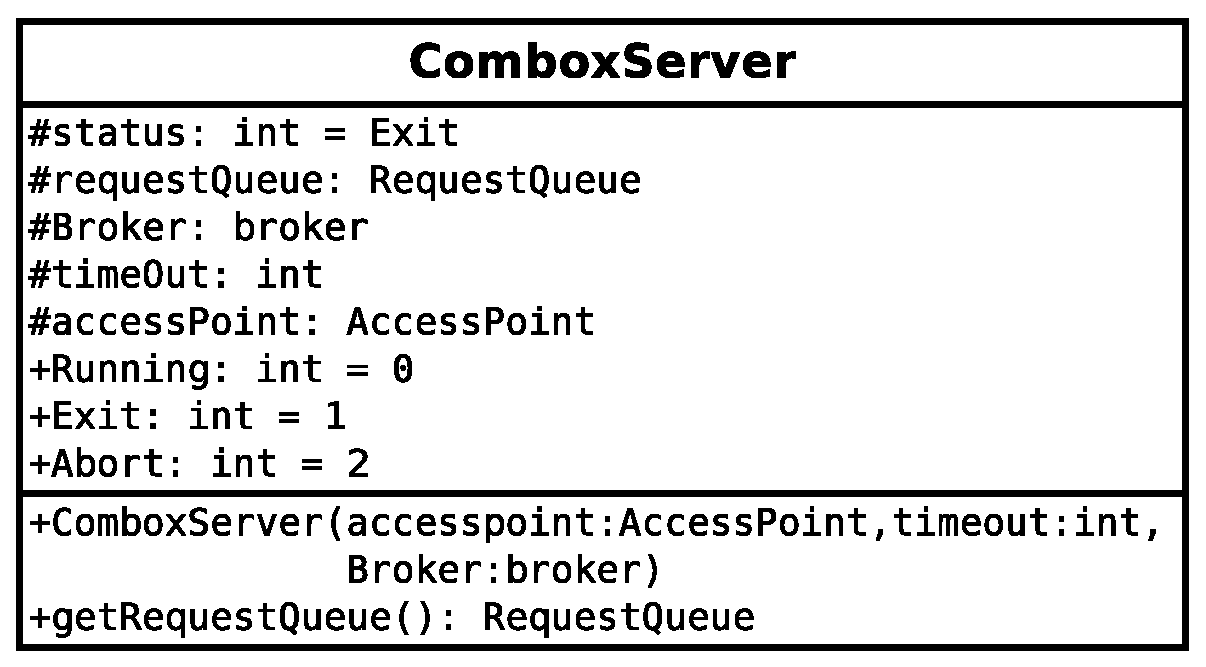
\includegraphics[scale=0.5]{comboxserver.eps}
\end{figure}

The combox factory must inherits from the super class ComboxFactory located in the package popjava.combox in the POP-Java library. The figure[\ref{fig:comboxfactory_class}] shows the ComboxFactory class signature.

\begin{figure}[ht]
\caption{ComboxFactory class signature}
\center
\label{fig:comboxfactory_class}
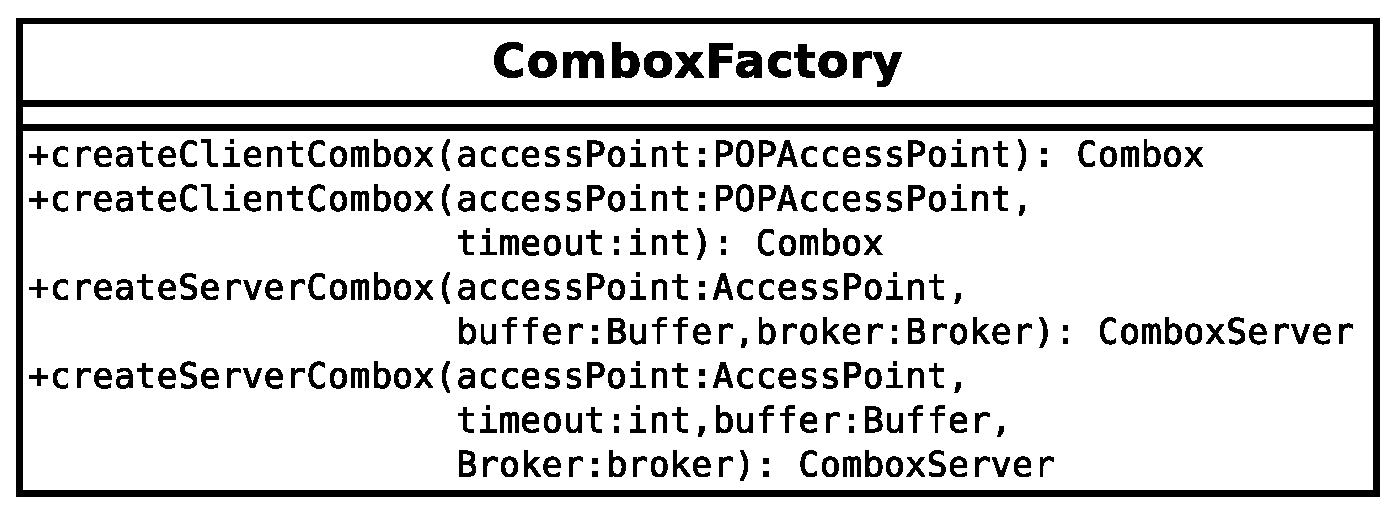
\includegraphics[scale=0.5]{comboxfactory.eps}
\end{figure}


Once all the classes are implemented, the programmer needs to compile them as standard Java code and create a JAR file. This JAR file can be added in the system by editing the file pop\_combox.xml located in the directory \textit{POPJAVA\_LOCATION/plugin}. The XML code below is the current XML file with the socket protocol.

\begin{lstlisting}
<ComboxFactoryList>
  <Package JarFile="popjava.combox.jar">
    <ComboxFactory>popjava.combox.ComboxSocketFactory</ComboxFactory>
  </Package>
</ComboxFactoryList>
\end{lstlisting}


\pagebreak
\subsection{Buffer plugin}
The buffer is the component in charge of the data encoding. In the current implementation of POP-Java, two buffers are available. One is using the RAW encoding and the other is using the XDR encoding. If the programmer needs a special encoding protocol, he can also create his own and add it to the POP-Java system as a plugin. \s

To implement a new encoding protocol, the programmer needs to create two class. A buffer and a buffer factory. \s

The buffer must inherits from the super class BufferPlugin located in the package popjava.buffer in the POP-Java library. The figure[\ref{fig:buffer_class}] shows the BufferPlugin class signature.
\begin{figure}[ht]
\caption{BufferPlugin class signature}
\center
\label{fig:buffer_class}
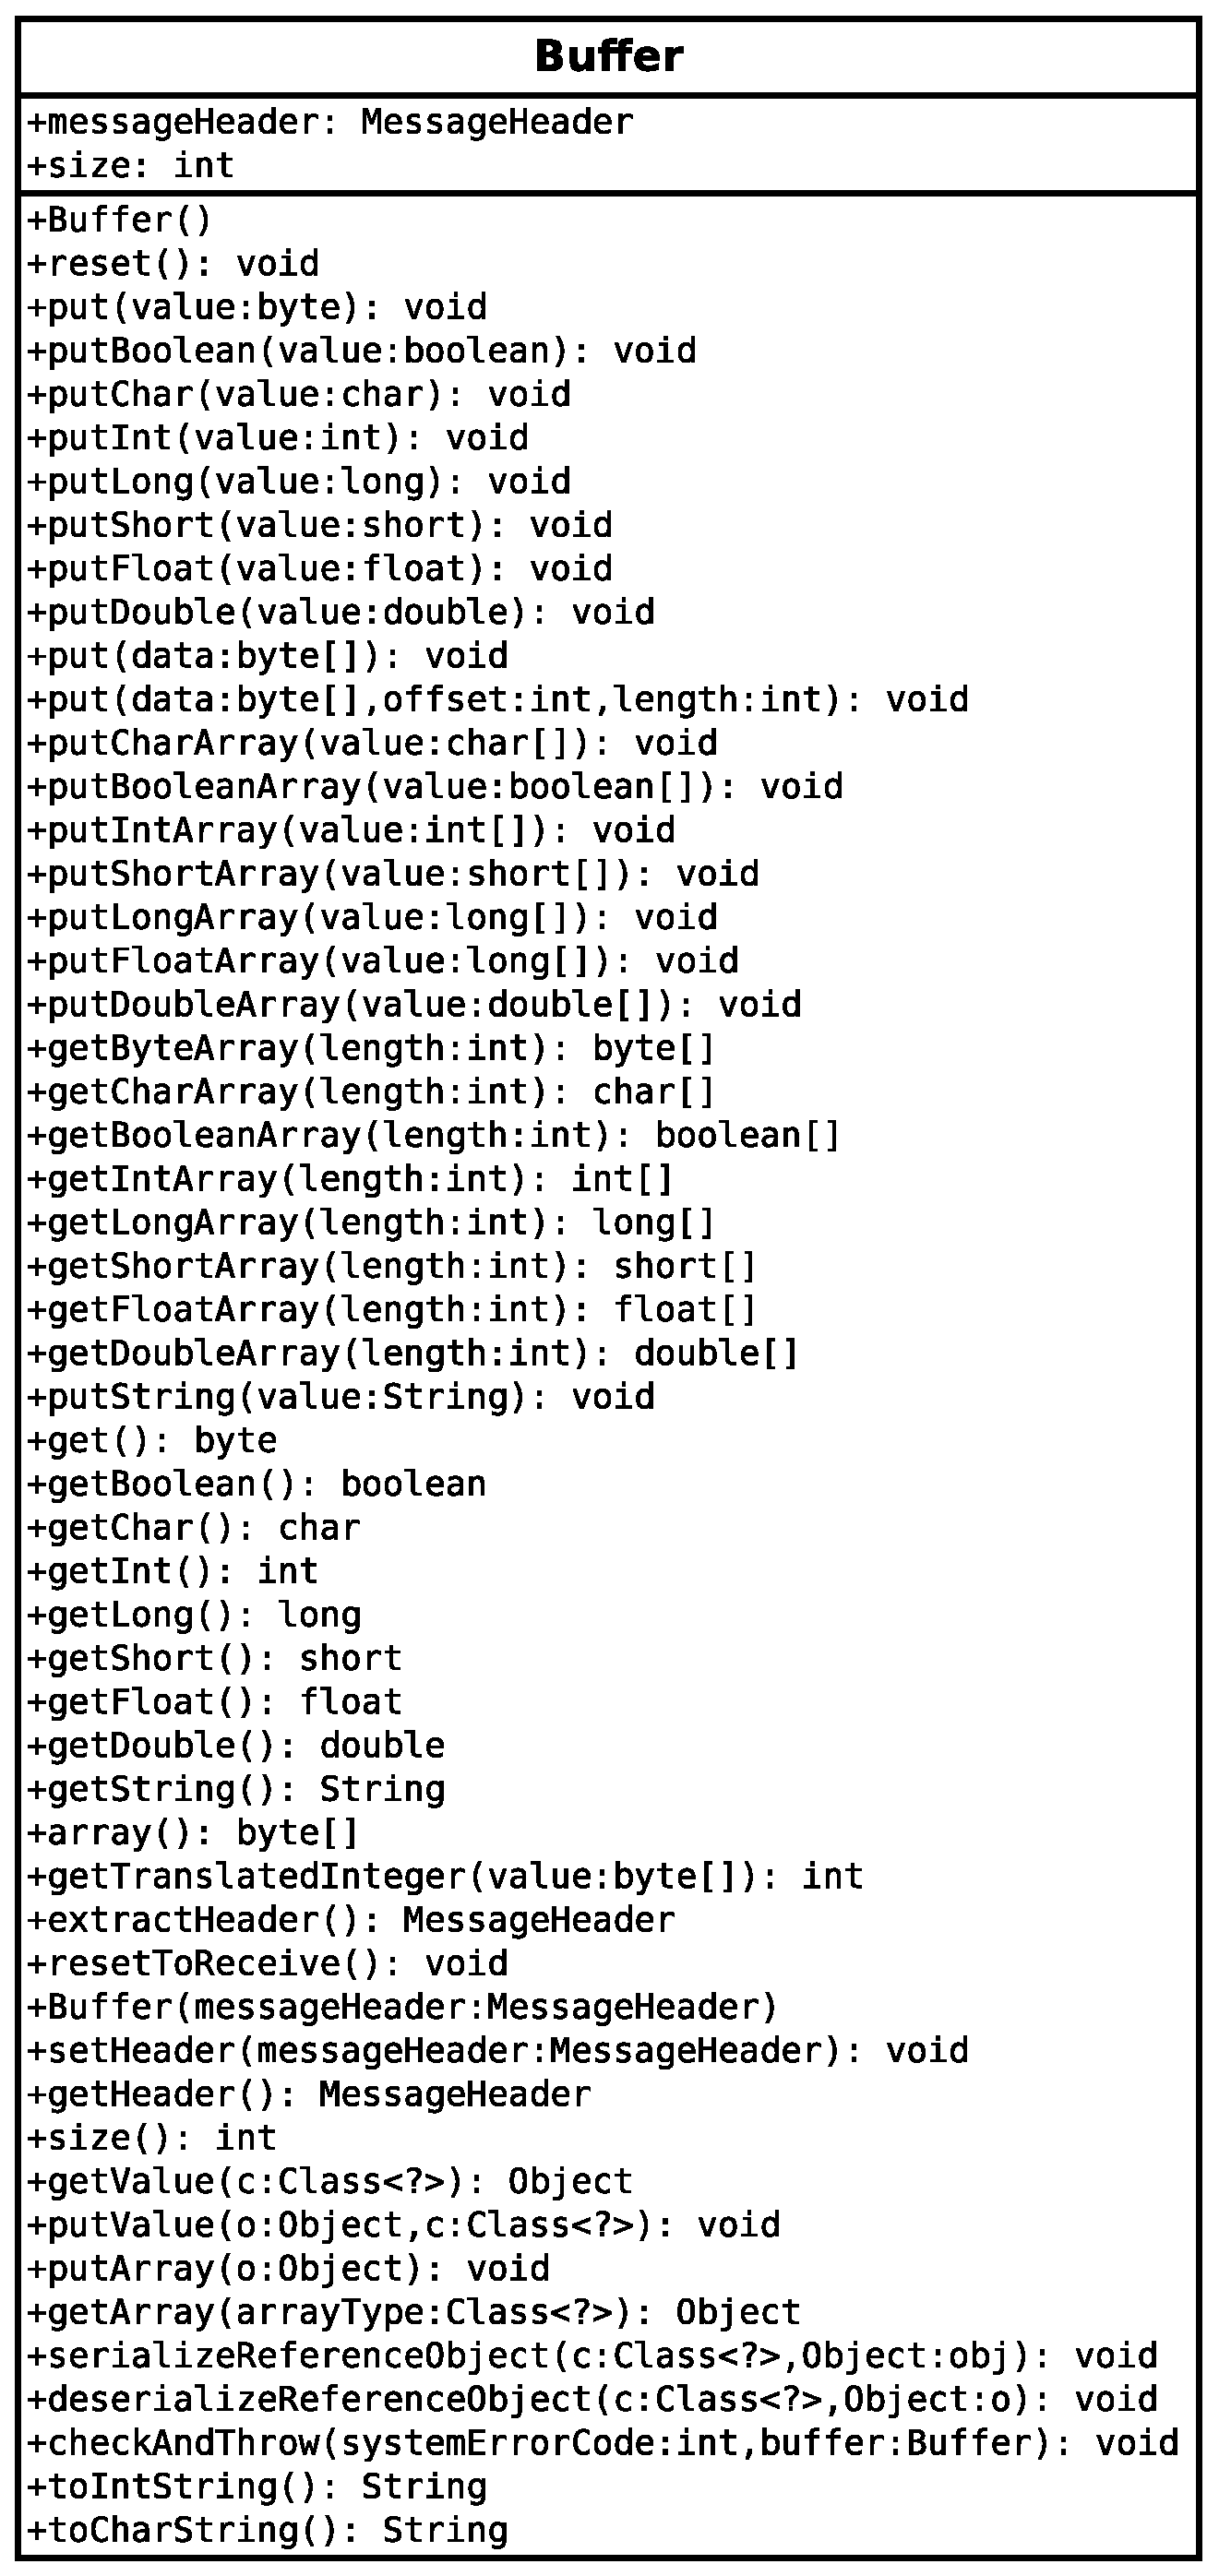
\includegraphics[scale=0.35]{buffer.eps}
\end{figure}

\pagebreak
The buffer factory must inherits from the super class BufferFactory located in the package popjava.buffer in the POP-Java library. The figure[\ref{fig:bufferfactory_class}] shows the BufferFactory class signature.
\begin{figure}[ht]
\caption{BufferFactory class signature}
\center
\label{fig:bufferfactory_class}
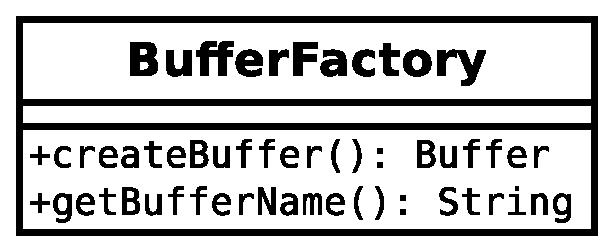
\includegraphics[scale=0.5]{bufferfactory.eps}
\end{figure}

